% !Mode:: "TeX:UTF-8"
% VL 2, gebaut aus part-grundlagen/02-neuron-perzeptron.md und 03-perzeptron-trainieren.md
% (Dialogmuster und Zeiten: transcripts/vl02-perzeptron-2025/notiz.md).
%
% Wenig Text auf den Folien, die Ausführung steht in \note{}.
% !Mode:: "TeX:UTF-8"
\newcommand{\thepage}{} % to silence a hyperref warning about pdfpagelabels
\RequirePackage[]{silence}
\WarningsOff[hyperref]
\PassOptionsToPackage{log-declarations=false}{xparse}
%\RequirePackage[l2tabu, orthodox]{nag}
\RequirePackage{luatex85} % to make \pdf...= commands work with LuaTeX
\documentclass[aspectratio=169,t]{beamer}
\usepackage{ifthen}
\usepackage[T1]{fontenc}
\usepackage{iftex}
\ifLuaTeX
 \usepackage{fontspec}
 \setmainfont[Ligatures=TeX]{Source Sans Pro}
\else
 \usepackage[utf8]{inputenc}
\fi
\usepackage{german}
\usepackage{newunicodechar}
\newunicodechar{€}{\texteuro}
\newunicodechar{ß}{\ss}
\renewcommand{\SS}{\iffontchar\font"1E9E \symbol{"1E9E}\else SS\fi}
\usepackage{ellipsis}
\usepackage{microtype}
\usepackage{listings}
\usepackage{sourcecodepro}
\lstset{language=Python, basicstyle=\ttfamily}
\usepackage{amsfonts}
\usepackage{amssymb}
\usepackage{amsthm}
\usepackage{fancyhdr}
\usepackage{graphicx}

\newtheorem{proposition}[theorem]{Proposition}

\DeclareMathOperator*{\argmax}{argmax}
\DeclareMathOperator{\supp}{supp}
\newcommand{\E}{\ensuremath{\mathbb{E}}}
\newcommand{\V}{\ensuremath{\mathbb{V}}}

\setbeamercolor{emph}{fg=purple}
\renewcommand<>{\emph}[1]{%
  {\usebeamercolor[fg]{emph}\only#2{\itshape}#1}%
}



\hypersetup{draft=false,colorlinks=false,pdfpagemode=UseOutlines,plainpages=false,
            breaklinks=true,bookmarksnumbered=true,pdfborder=0 0 0,
            pdftitle={Einführung in Deep Learning WiSe 2026/27 HHU},
            pdfauthor={Konrad Voelkel},
            pdfsubject={data science}}

%\documentclass[aspectratio=169,t]{beamer}
\usetheme{hhubeamer} % put the hhu-beamer-theme in /usr/share/texmf/tex/latex/beamer/themes/

% -------------------- Code listings config --------------------
% Define custom colors for syntax highlighting
\definecolor{codegreen}{rgb}{0,0.6,0}
\definecolor{codegray}{rgb}{0.5,0.5,0.5}
\definecolor{codepurple}{rgb}{0.58,0,0.82}
\definecolor{backcolour}{rgb}{0.96,0.96,0.94} % Very light gray/beige
% Configure the listings package
\lstset{
    language=Python,
    backgroundcolor=\color{backcolour},   
    commentstyle=\color{codegreen}\itshape,
    keywordstyle=\color{blue}\bfseries,
    numberstyle=\tiny\color{codegray},
    stringstyle=\color{codepurple},
    basicstyle=\ttfamily\footnotesize, % Use a monospaced font
    breakatwhitespace=false,         
    breaklines=true,      
             % Enable automatic line breaking
    captionpos=b,                      % Caption at the bottom
    keepspaces=true,                 
    numbers=left,                      % Line numbers on the left
    numbersep=10pt,                    % Distance of line numbers from the code
    showspaces=false,                
    showstringspaces=false,            % Don't show weird underscores in strings
    showtabs=false,                  
    tabsize=4,
    frame=single,                      % Add a subtle border around the code
    rulecolor=\color{black!20},        % Border color
  }

\event[]{}
\author[Wintersemester 2026/27]{Dr. Konrad Völkel, Wintersemester 2026/27}

%\title{Data Science, VL 1}
%\date{16.04.2026}


%%% Local Variables:
%%% mode: latex
%%% TeX-master: t
%%% End:


% Fassung mit Dozentennotizen (zweiter Schirm): die nächste Zeile einkommentieren.
% \setbeameroption{show notes on second screen=right}

\graphicspath{{../images/}}

\title[Neuron und Perzeptron (VL 2)]{Neuron und Perzeptron\\\large Einführung in Deep Learning, VL 2}
\date{21.10.2026}

\begin{document}

\begin{frame}
  \titlepage

  \note{\textbf{Ablauf, 90 Minuten} (2025: 60 Min. Folien, 15 Min. Tafel, 13 Min. Dialog):\\[2pt]
    \begin{tabular}{@{}rll@{}}
      0--5   & Folie 2       & Rückblick, erstes Blatt ist abgegeben\\
      5--15  & Folien 3--4   & McCulloch-Pitts-Neuron, Kochrezept\\
      15--28 & Folien 5--7   & Perzeptron, Bias-Trick, Geometrie \textbf{(Tafel)}\\
      28--35 & Folien 8--9   & Abstand, Skalierung von $w$\\
      35--45 & Folien 10--11 & Linear trennbar, XOR\\
      45--52 & Folie 12      & Die fünf Fragen an jedes Modell\\
      52--62 & Folien 13--14 & Perzeptronregel\\
      62--75 & Folie 15      & \textbf{Tafel: warum sie für ein Sample funktioniert}\\
      75--82 & Folien 16--17 & Verallgemeinertes Perzeptron\\
      82--88 & Folien 18--19 & Mehrere Schichten, warum die Regel nicht reicht\\
      88--90 & Folie 20      & Übungsblatt\\
    \end{tabular}\\[4pt]
    Die Tafelphase ist der Kern der Sitzung -- 2025 war das Ein-Sample-Argument das,
    was der Dozent am Ende „das Wichtigste“ genannt hat. Wenn die Zeit knapp wird:
    Konvergenzsatz (Folie 16) weglassen, er steht als Vertiefung im Skript.}
\end{frame}

% ------------------------------------------------------------------ Rückblick
\begin{frame}
  \frametitle{Wo wir stehen}

  \begin{center}
    \Large Letzte Woche: \emph{was} Deep Learning ist.\\[12pt]
    Heute: das kleinste Netz -- ein einziges Neuron.
  \end{center}

  \note{Zwei Sätze Rückblick, mehr nicht. Ansagen: das erste Blatt war heute 12:00 fällig,
    das nächste kommt raus und implementiert die Perzeptronregel.
    Wer letzte Woche nicht da war: Kapitel 1 im Skript, zehn Minuten Lesezeit.}
\end{frame}

% ------------------------------------------------------------------ Neuron
\begin{frame}
  \frametitle{Das McCulloch-Pitts-Neuron (1943)}

  \begin{columns}[c]
    \begin{column}{0.48\textwidth}
      \begin{center}
        \Large
        $\zeta = \sum_{j=1}^n w_j x_j = w \cdot x$\\[16pt]
        $y = \sigma(\zeta)$
      \end{center}
    \end{column}
    \begin{column}{0.48\textwidth}
      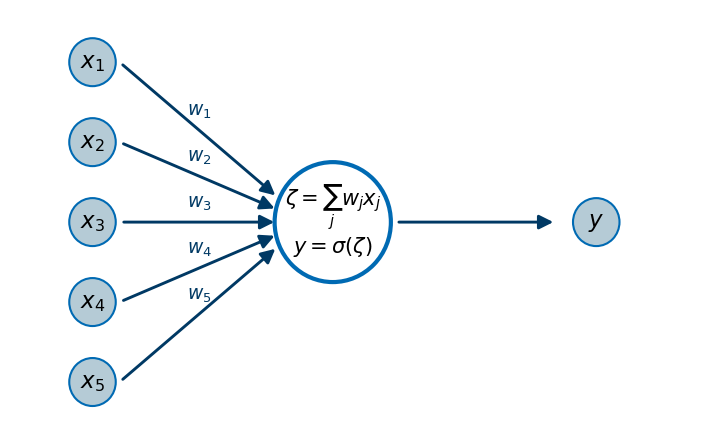
\includegraphics[width=\textwidth]{vl01-neuron.png}
    \end{column}
  \end{columns}

  \note{Von der Biologie geborgt: Dendriten liefern Signale, das Neuron summiert sie
    gewichtet und feuert, wenn eine Schwelle überschritten wird.
    Bei McCulloch und Pitts ist $\sigma$ eine Schwellenwertfunktion mit Ausgabe 0 oder 1;
    später wird daraus Sigmoid oder ReLU.
    \textbf{Type-Check als Stilmittel} (hat 2025 gut getragen): Was für ein Objekt ist $w$,
    was $x$, was $\zeta$? Aus den Typen folgt, dass $\sigma$ von $\mathbb{R}$ nach
    $\mathbb{R}$ geht.}
\end{frame}

\begin{frame}
  \frametitle{Das Kochrezept}

  \begin{center}
    \Huge Skalarprodukt,\\[8pt] dann etwas Nichtlineares.
  \end{center}

  \note{Diese Folie ist die Take-Home-Message des Semesters, nicht nur der Sitzung.
    Alles, was wir bauen -- logistische Regression, MLP, CNN, Transformer -- ist eine
    Variation davon. Und am Ende der Sitzung sehen wir: ohne das Nichtlineare bringt
    Stapeln gar nichts.}
\end{frame}

% ------------------------------------------------------------------ Perzeptron
\begin{frame}
  \frametitle{Das Perzeptron (Rosenblatt 1958)}

  \begin{center}
    \Large $f(x) = [\, w \cdot x + b > 0 \,]$
  \end{center}

  \bigskip
  \begin{itemize}
  \item binäre Klassifikation: $X \in \mathbb{R}^n$, $Y \in \{0,1\}$
  \item Parameter: $w \in \mathbb{R}^n$ und $b \in \mathbb{R}$
  \item $[\cdot]$ ist die Iverson-Klammer
  \end{itemize}

  \note{Rosenblatts Beitrag war weniger das Neuron als der \emph{Lernalgorithmus} dafür --
    dazu kommen wir in der zweiten Hälfte.
    Wichtig hier: $f$ ist \emph{nichtlinear}, obwohl innen nur ein Skalarprodukt steht.
    Das ist ein beliebter Denkfehler.}
\end{frame}

\begin{frame}
  \frametitle{Der Bias-Trick}

  \begin{center}
    \Large
    $w_0 := b$, \quad $x_0 := 1$\\[14pt]
    $\Longrightarrow\quad w \cdot x + b = \sum_{j=0}^n w_j x_j$
  \end{center}

  \note{Ab jetzt schreiben wir kurz $f(x) = [\,w \cdot x > 0\,]$ und denken uns den Bias
    als nulltes Gewicht. Diesen Trick sehen wir noch öfter.
    Rückfrage in den Raum: Was kann ein Perzeptron \emph{ohne} Bias nicht?
    Antwort: nur Hyperebenen durch den Ursprung -- zwei Klassen, die eine verschobene
    Gerade brauchen, bleiben ihm verschlossen. 2025 kam dazu das Tafelbild mit den zwei
    Clustern.}
\end{frame}

\begin{frame}
  \frametitle{$w$ steht senkrecht auf der Trenngeraden}

  \begin{center}
    \Large $w \cdot (x - x') = (w \cdot x + b) - (w \cdot x' + b) = 0$
  \end{center}

  \bigskip
  \begin{center}
    für alle $x, x'$ auf der Hyperebene $H = \{ w \cdot x + b = 0\}$.
  \end{center}

  \note{\textbf{Tafel.} Gerade zeichnen, $w$ als Pfeil senkrecht darauf, einen Punkt
    daneben. Die Rechnung ist drei Zeilen und überzeugt sofort.
    In $\mathbb{R}^2$ ist $H$ eine Gerade, in $\mathbb{R}^n$ eine Hyperebene; $f$ sagt nur,
    auf welcher Seite $x$ liegt.}
\end{frame}

\begin{frame}
  \frametitle{Die Aktivierung ist der Abstand}

  \begin{center}
    \Large
    $x = x_H + d\,\tilde{w}$, \quad $\tilde{w} = w/\|w\|$\\[14pt]
    $d = \dfrac{w \cdot x + b}{\|w\|}$
  \end{center}

  \bigskip
  \begin{center}
    vorzeichenbehaftet: positiv auf der Seite, in die $w$ zeigt.
  \end{center}

  \note{Das ist die Aussage, die den Rest des Semesters trägt: Die Aktivierung eines
    Neurons ist der Abstand zur Hyperebene, mal $\|w\|$.
    Beispiel zum Mitrechnen: $w = (3,4)$, $b = -5$, also $\|w\| = 5$. Punkt $(1,\frac12)$
    liegt auf $H$. Punkt $(3,4)$: Aktivierung $9+16-5 = 20$, Abstand $4$. Punkt $(-1,0)$:
    Aktivierung $-8$, Abstand $-8/5$, andere Seite. Das ist eine Übungsaufgabe.}
\end{frame}

\begin{frame}
  \frametitle{Richtung und Länge von $w$}

  \begin{center}
    \Large
    $w \mapsto c\,w$, \quad $b \mapsto c\,b$ \quad $(c > 0)$\\[14pt]
    \normalsize
    dieselbe Gerade, dieselbe Entscheidung\\[6pt]
    aber: Aktivierung mal $c$
  \end{center}

  \note{Für das Perzeptron ist die Länge egal. Sobald die Aktivierungsfunktion glatt ist,
    ist sie es nicht mehr: $\sigma(10 \cdot 20)$ ist praktisch 1, $\sigma(0{,}01 \cdot 20)$
    nur knapp über $\frac12$. Dieselbe Trenngerade, ganz andere „Sicherheit“.
    Das kommt in VL 4 wieder, wenn aus der Aktivierung eine Wahrscheinlichkeit wird --
    hier nur ankündigen.}
\end{frame}

% ------------------------------------------------------------------ Grenzen
\begin{frame}
  \frametitle{Linear trennbar}

  \begin{center}
    $A, B \subseteq \mathbb{R}^n$ heißen \emph{linear trennbar}, wenn es $w, b$ gibt mit\\[10pt]
    \Large
    $w \cdot a + b > 0$ für alle $a \in A$,\\[6pt]
    $w \cdot a' + b \le 0$ für alle $a' \in B$.
  \end{center}

  \note{Ein Perzeptron kann genau die Probleme lösen, bei denen die Klassen linear
    trennbar sind -- nicht mehr.}
\end{frame}

\begin{frame}
  \frametitle{Das Gegenbeispiel: XOR}

  \begin{center}
    \Large
    $(0,0), (1,1) \quad\longleftrightarrow\quad (0,1), (1,0)$\\[18pt]
    \normalsize Keine Gerade trennt diese beiden Paare.
  \end{center}

  \note{An die Tafel zeichnen, vier Punkte, zwei Farben -- dann versuchen zu trennen.
    Das ist die mathematische Substanz hinter dem AI Winter aus der letzten Woche,
    und der Grund, warum wir Neuronen hintereinanderschalten werden.
    Auflösung kommt am Ende der Sitzung.}
\end{frame}

% ------------------------------------------------------------------ Modellfragen
\begin{frame}
  \frametitle{Fünf Fragen an jedes Modell}

  \begin{enumerate}\setlength{\itemsep}{6pt}
  \item Was sind die freien Parameter?
  \item Wie läuft die Inferenz?
  \item Wie funktioniert das Training?
  \item Was ist die Zielgröße -- wann ist genug trainiert?
  \item Welche Hyperparameter gibt es?
  \end{enumerate}

  \note{Diese fünf Fragen kommen bei jedem Modell dieser Vorlesung wieder; es lohnt sich,
    sie mitzuschreiben.
    2025 kam hier die Frage, was Parameter von Hyperparametern unterscheidet:
    Parameter werden gelernt, Hyperparameter werden gewählt. Die Dimension $n$ ist ein
    Hyperparameter, den die Daten vorgeben.}
\end{frame}

% ------------------------------------------------------------------ Perzeptronregel
\begin{frame}
  \frametitle{Die Perzeptronregel}

  \begin{center}
    \Huge $w_{\text{neu}} := w + \rho\,(y - f(x))\,x$
  \end{center}

  \note{$\rho > 0$ ist die Lernrate, ein Hyperparameter.
    Type-Check: Was muss $\rho$ sein, damit die Formel Sinn ergibt? Ein Skalar.
    Und $(y - f(x))$? Eine Zahl aus $\{-1, 0, 1\}$.}
\end{frame}

\begin{frame}
  \frametitle{Drei Fälle}

  % description statt itemize: Beamer schneidet lange \item[...]-Labels links ab.
  \begin{description}[$y = 1,\ f(x) = 0$]\setlength{\itemsep}{10pt}
  \item[$y = f(x)$] nichts passiert
  \item[$y = 1,\ f(x) = 0$] $w_{\text{neu}} = w + \rho x$, Aktivierung wächst
  \item[$y = 0,\ f(x) = 1$] $w_{\text{neu}} = w - \rho x$, Aktivierung sinkt
  \end{description}

  \note{Der mittlere Fall zum Mitrechnen: $w_{\text{neu}} \cdot x = w \cdot x + \rho\,(x \cdot x)$,
    und $x \cdot x > 0$ für $x \neq 0$. Die Aktivierung wächst also -- in Richtung der
    richtigen Entscheidung.
    Frage in den Raum, die 2025 kam: Muss eine Änderung a priori verbessern? Nein --
    für \emph{dieses} Sample ja, für andere kann sie es verschlechtern.}
\end{frame}

\begin{frame}
  \frametitle{Warum das funktioniert}

  \begin{center}
    \Huge $w^{(k)} \cdot x = w^{(0)} \cdot x + k\,\rho\,\|x\|^2$
  \end{center}

  \note{\textbf{Das ist die Tafelphase, 10--15 Minuten -- der Kern der Sitzung.}
    Die Formel steht hier, hergeleitet wird sie an der Tafel aus der Bilinearität des
    Skalarprodukts. Für großes $k$ wird der Ausdruck positiv, egal wie schlecht
    $w^{(0)}$ war.
    Dazu das Winkelbild: jedes Update addiert ein Vielfaches von $x$ zu $w$, dreht $w$
    also in Richtung $x$ (bei $y = 0$ von $x$ weg); die Entscheidungsgrenze steht
    senkrecht auf $w$ und dreht sich mit.
    Ausdrücklich sagen: Das ist die eine Rechnung, die man einmal selbst auf Papier
    gemacht haben sollte (steht auf einem Übungsblatt).
    Einschränkung nennen: Ein Update für $x$ kann ein anderes $x'$ auf die falsche Seite
    schieben -- dass das endet, ist der Konvergenzsatz.}
\end{frame}

\begin{frame}
  \frametitle{Die Regel bei der Arbeit}

  \begin{center}
    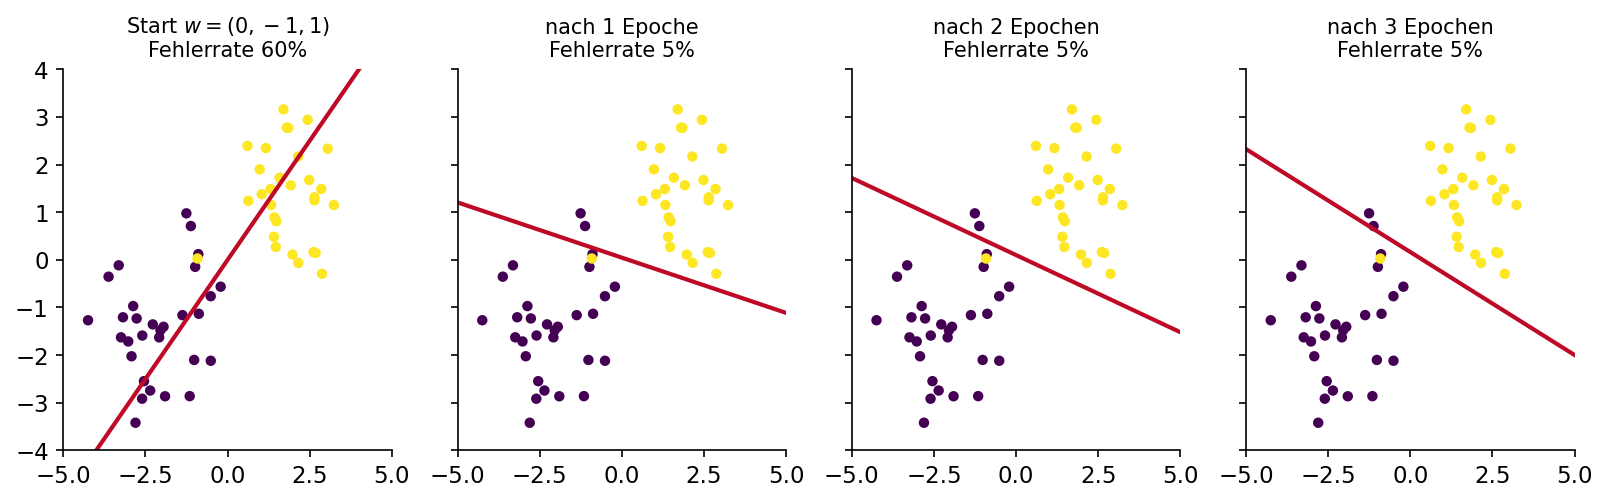
\includegraphics[width=0.8\textwidth]{vl02-perceptron-updates.png}
  \end{center}

  \note{Trenngerade nach 0, 1, 2 und 3 Epochen über 60 Datenpunkte, Lernrate $\rho = 0{,}05$.
    Genau das baut das Übungsblatt nach.
    Hier den Konvergenzsatz nur beim Namen nennen (Novikoff 1962): höchstens
    $R^2/\gamma^2$ Fehler, wenn es eine Margin $\gamma$ gibt. Der Beweis steht als
    Vertiefung im Skript.}
\end{frame}

% ------------------------------------------------------------------ Verallgemeinerung
\begin{frame}
  \frametitle{Verallgemeinertes Perzeptron}

  \begin{center}
    \Large $f(x) = \tau(w \cdot x)$
  \end{center}

  \bigskip
  \begin{center}
    \begin{tabular}{@{}lll@{}}
      \textbf{Modell} & $\tau(a)$ & \textbf{Training}\\[3pt]
      Lineare Regression & $a$ & kleinste Quadrate\\
      Perzeptron & $[a > 0]$ & Perzeptronregel\\
      „stetiges Perzeptron“ & $\tanh(a)$ & \emph{?}\\
      Logistische Regression & $\sigma(a)$ & \emph{?}\\
    \end{tabular}
  \end{center}

  \note{Die beiden Fragezeichen sind das Programm der nächsten Wochen: Gradientenabstieg
    auf einer Loss-Funktion (VL 5), und die Perzeptronregel wird sich als Spezialfall
    erweisen (Übungsblatt).
    Die letzten beiden $\tau$ sind glatte Versionen der Sprungfunktion: $\tanh$ nach
    $(-1,1)$, $\sigma$ nach $(0,1)$.}
\end{frame}

\begin{frame}
  \frametitle{Mehrere Schichten: das MLP}

  \begin{columns}[c]
    \begin{column}{0.46\textwidth}
      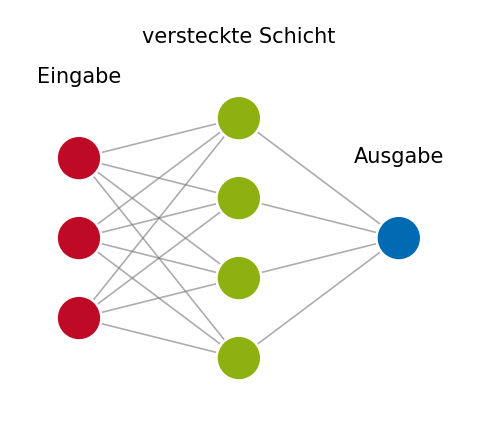
\includegraphics[width=\textwidth]{vl01-mlp.png}
    \end{column}
    \begin{column}{0.5\textwidth}
      \Large
      $h = \sigma(W x + b)$\\[14pt]
      \normalsize
      Zeile $i$ von $W$ = Gewichte von Neuron $i$
    \end{column}
  \end{columns}

  \note{Die $i$-te Komponente von $Wx$ ist das Skalarprodukt der $i$-ten \emph{Zeile} mit $x$.
    Also: $m$ Aktivierungen auf einmal -- mit der Geometrie von vorhin: $m$ skalierte
    Abstände zu $m$ Hyperebenen. Jedes Neuron zeichnet eine Gerade in die Eingabeebene.
    In PyTorch: \texttt{nn.Linear(n, m)} hat \texttt{weight} mit Shape \texttt{(m, n)}.
    Jetzt XOR auflösen: zwei Geraden in der ersten Schicht ($x_1 \lor x_2$ und
    $\lnot(x_1 \land x_2)$), ein UND darüber -- im Raum der Seiten-Informationen ist XOR
    linear trennbar.}
\end{frame}

\begin{frame}
  \frametitle{Zwei Probleme mit dem Stapeln}

  \begin{itemize}\setlength{\itemsep}{14pt}
  \item Die Perzeptronregel sagt nichts darüber, wie die \emph{vordere} Schicht angepasst wird.\\
    {\small Wer war schuld? $\longrightarrow$ Backpropagation (VL 6)}
  \item Ohne Nichtlinearität ist gestapelt dasselbe wie flach:\\
    {\small $u_1 (v \cdot x) + u_2 (w \cdot x) = (u_1 v + u_2 w) \cdot x$}
  \end{itemize}

  \note{Der zweite Punkt kurz vorrechnen -- er ist der Grund, warum $\tau$
    \emph{Aktivierungsfunktion} heißt und nicht Dekoration. Ein Produkt von Matrizen ist
    wieder eine Matrix.
    Der erste Punkt ist die Motivation für die nächsten Wochen: Backpropagation
    funktioniert nur für differenzierbare $\tau$ -- deshalb verabschieden wir uns von
    der Sprungfunktion.}
\end{frame}

% ------------------------------------------------------------------ Abschluss
\begin{frame}
  \frametitle{Übungsblatt}

  \begin{itemize}\setlength{\itemsep}{8pt}
  \item Perzeptronregel selbst implementieren (NumPy, nicht das verallgemeinerte Perzeptron)
  \item Zweidimensionale Daten wählen und \emph{plotten}
  \item Mehrere Epochen laufen lassen
  \end{itemize}

  \bigskip
  \begin{center}
    Nächste Woche: fertige Modelle benutzen -- und Tensoren.
  \end{center}

  \note{Ausdrücklich ansagen (hat 2025 Rückfragen erspart): mit \texttt{make\_blobs}
    anfangen, das ist der einfachste Fall; plotten, sonst sieht man nichts; mehrere
    Epochen. Der verlinkte Code ist Ugly Code und nur für den Notfall.
    Und: ChatGPT liefert hier Lehrbuchzeug, das nicht zur Aufgabe passt.}
\end{frame}

\end{document}

%%% Local Variables:
%%% mode: latex
%%% TeX-master: t
%%% End:
